\begin{figure}
    \begin{center}
        \subfloat[Mean reward per step over the last 20 episodes.]{
            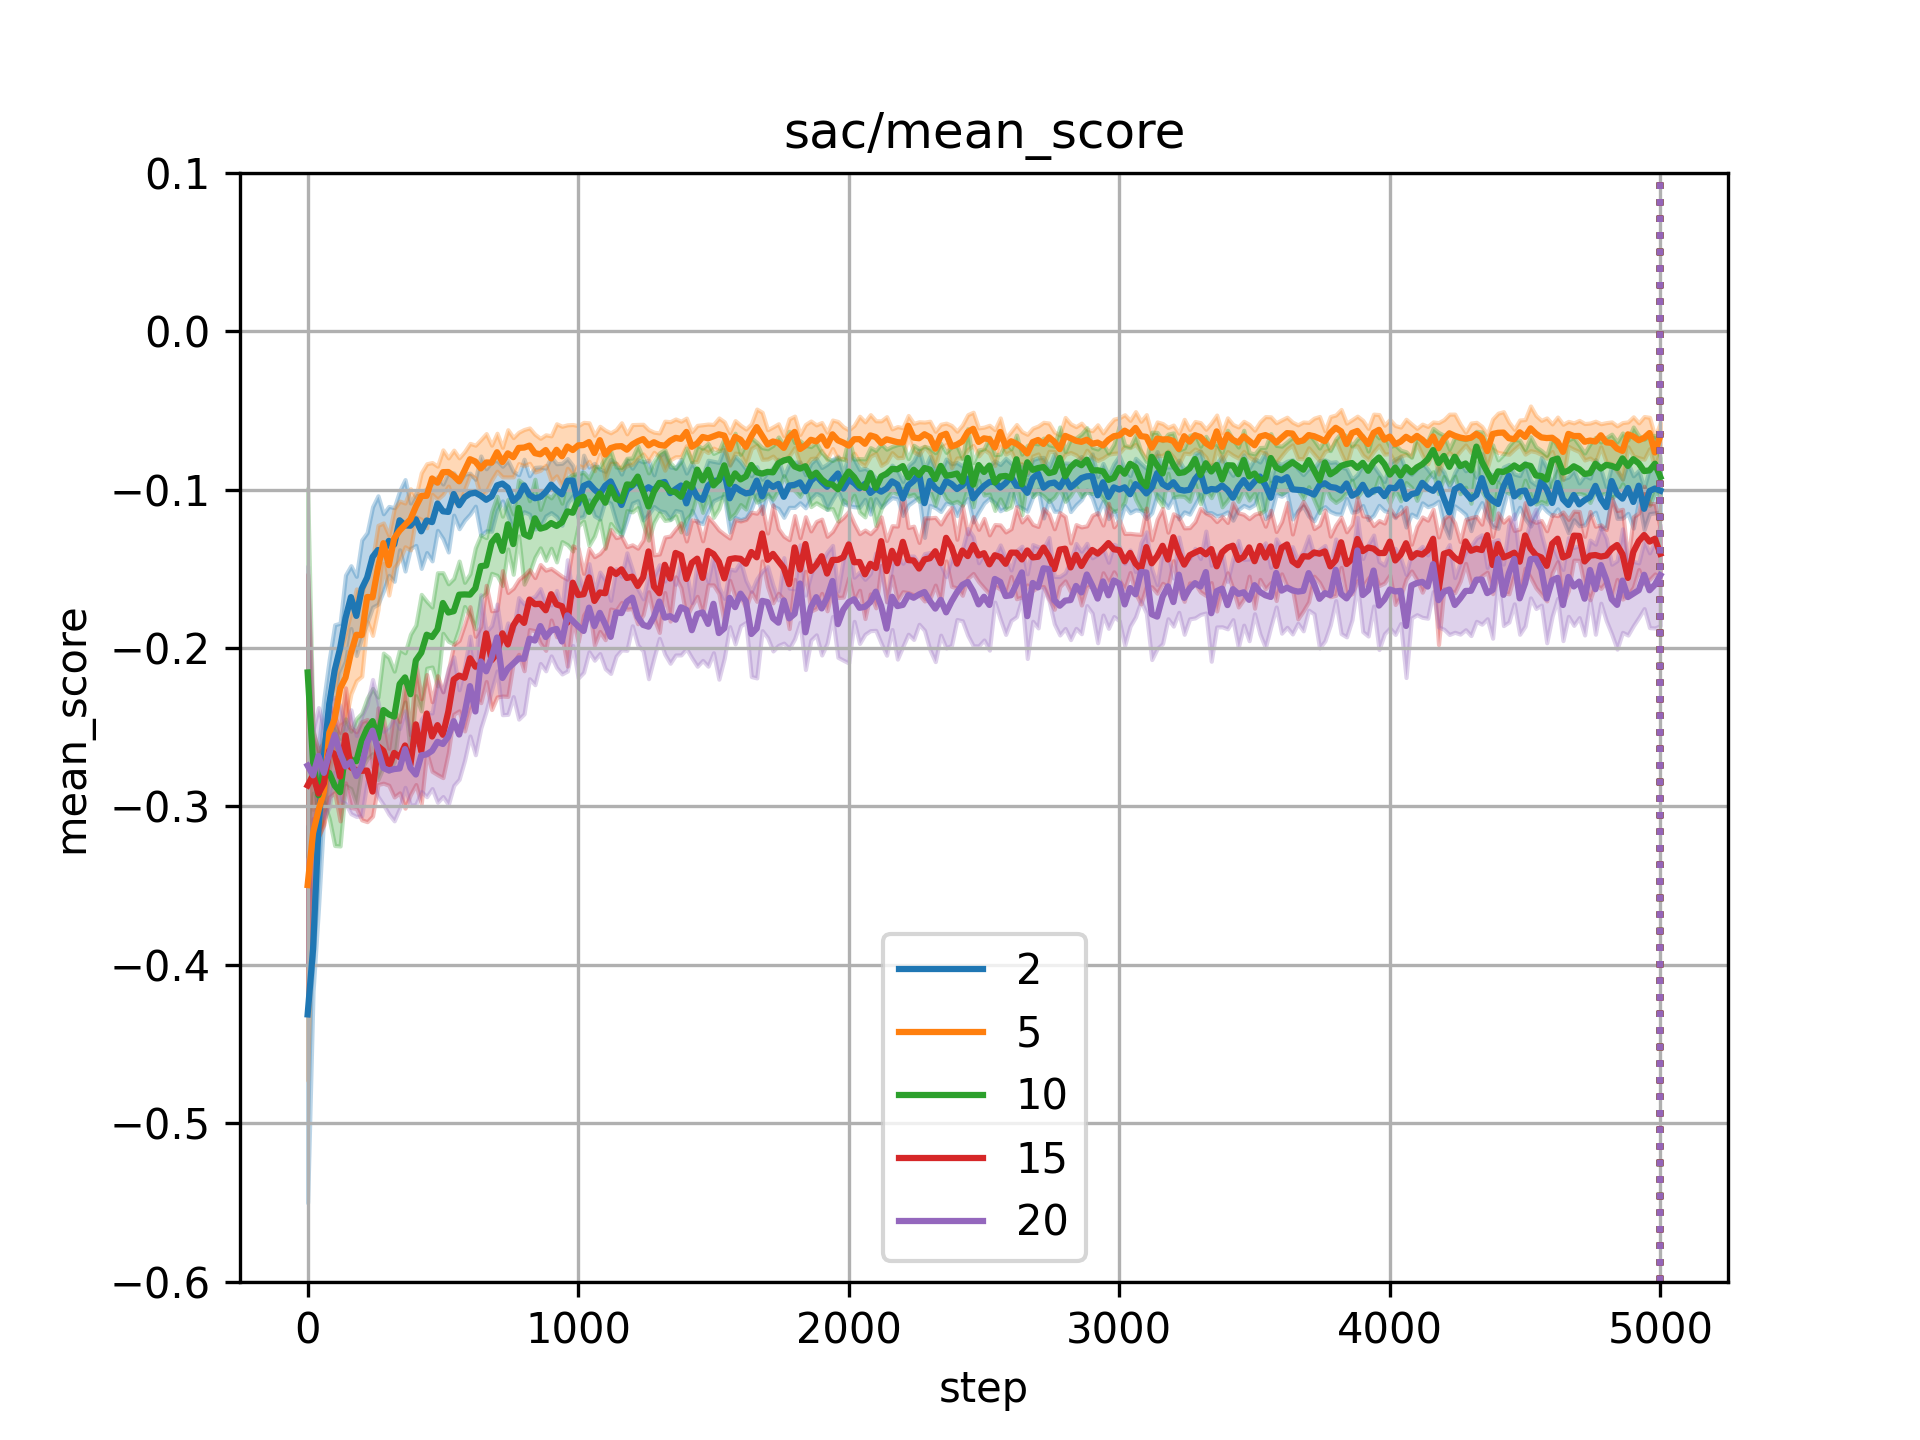
\includegraphics[width=0.46 \linewidth]{figures/experiments/sac_baseline_mean_score.png}
            \label{fig:SAC_baseline/reward}
            }
        \hfill
        \subfloat[Mean episode length over the last 20 episodes]{
        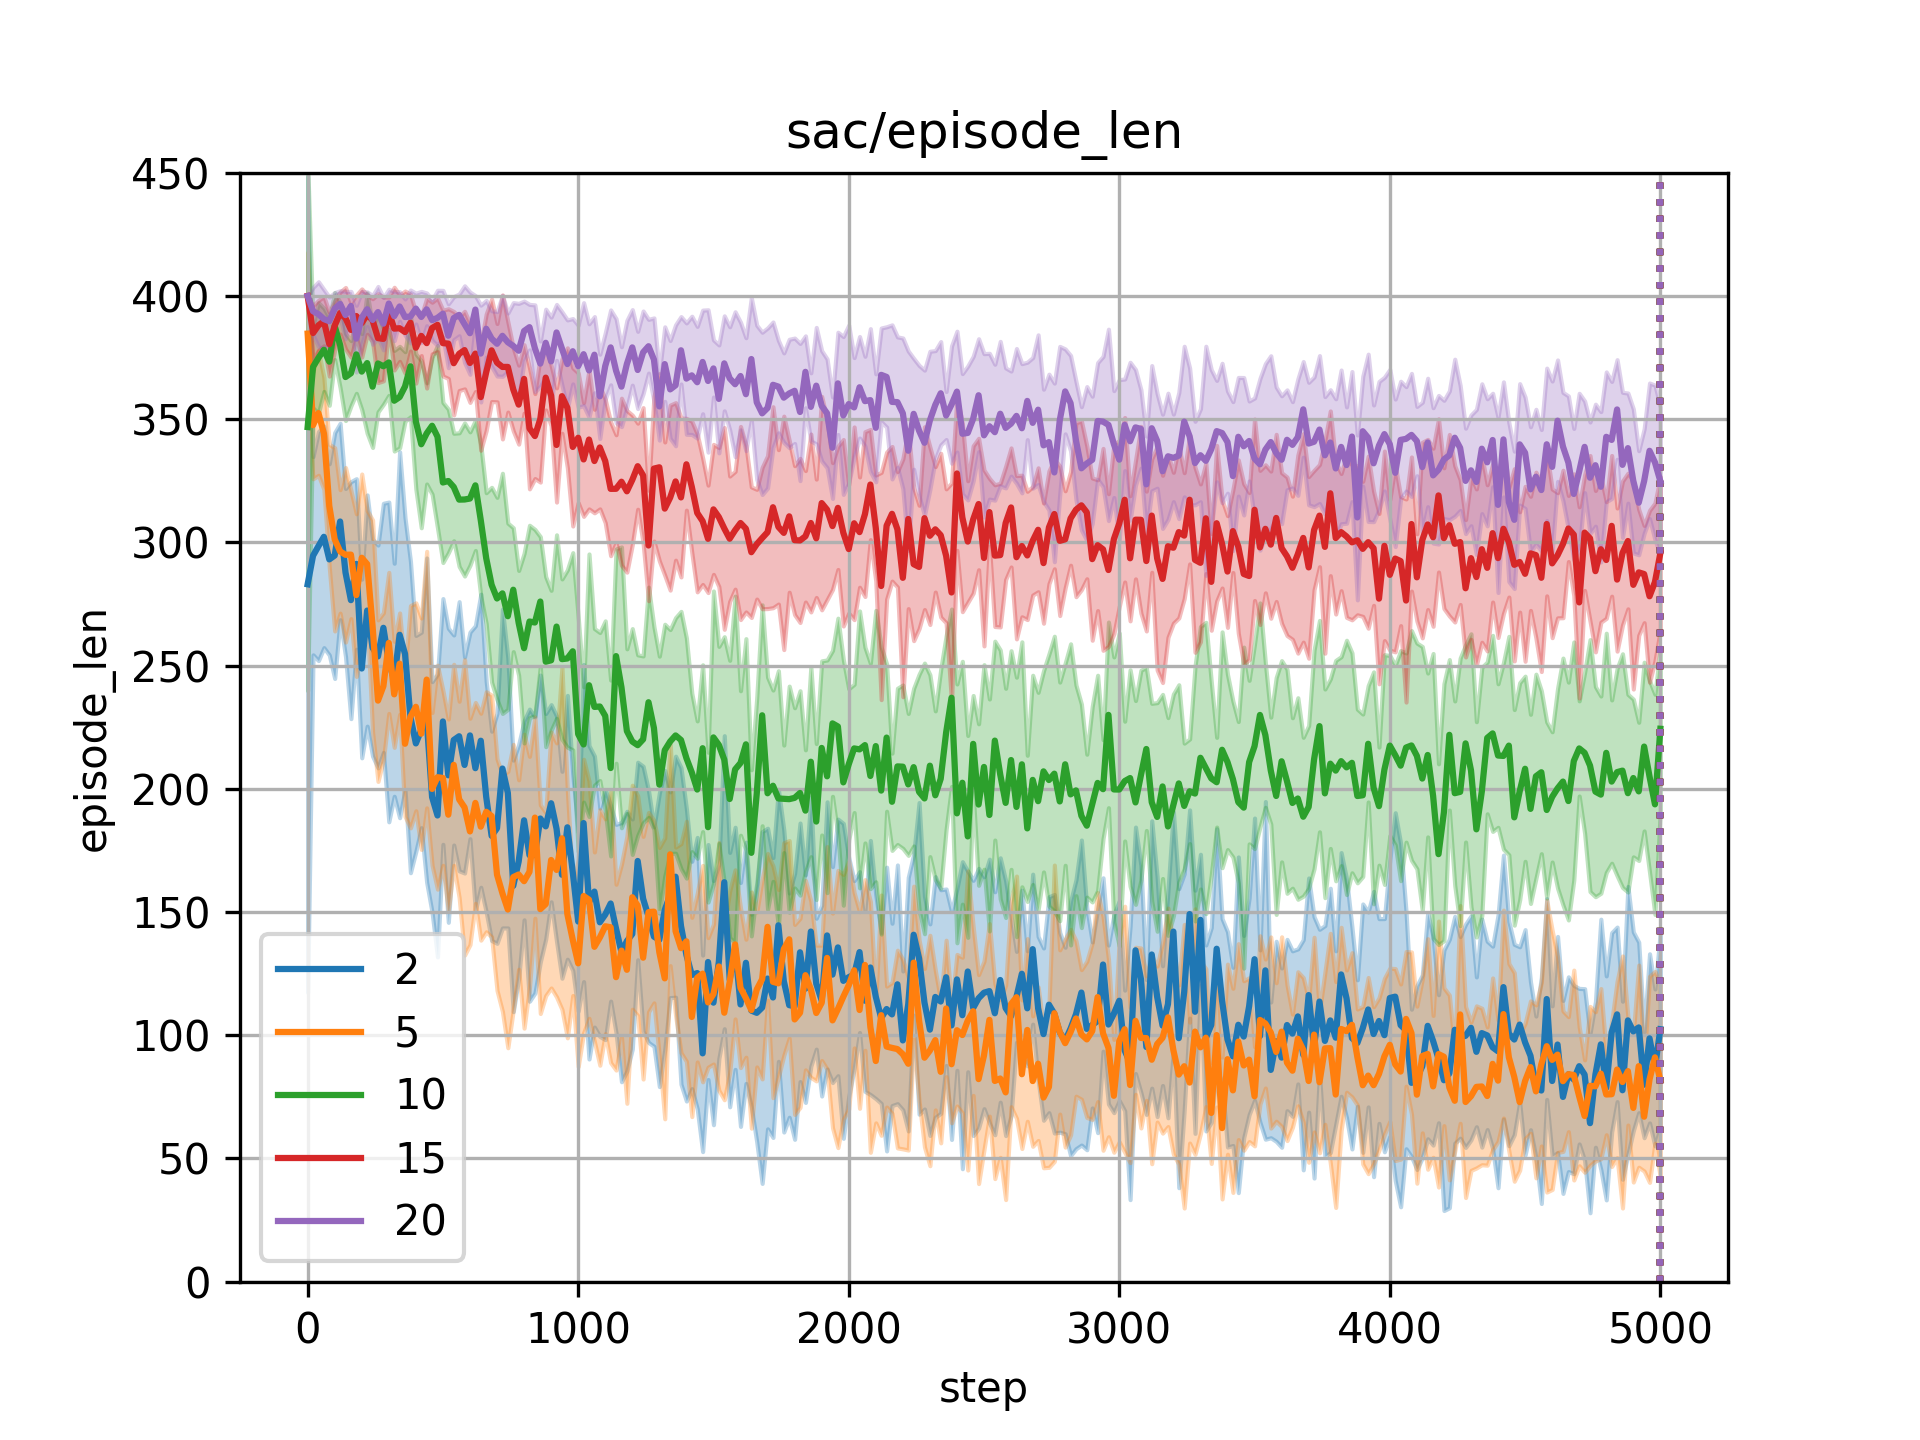
\includegraphics[width=0.46 \linewidth]{figures/experiments/sac_baseline_episode_len.png}
            \label{fig:SAC_baseline/episode_len}
            }
    \end{center}
    \caption[SAC baseline experiment results]{SAC baseline experiment results with an increasing number of joints. We can clearly see that the algorithm does not scale well with an increasing number of joints and therefor drops in performance. Each experiment was conducted 10 times and the shaded areas resemble the standard deviation around the mean.}
    \label{fig:SAC_baseline}
\end{figure}

